\section{Synthesis}

%Résumé des problématiques dans la littérature actuelle
The reliance of agriculture on irrigation has been rapidly increasing in the 20th century and is still on the rise. It is projected that irrigation demand will keep increasing in the future, especially as it is often regarded as an adaptation strategy to compensate for the effects of climate change, namely higher temperatures and disrupted precipitation patterns, and maintain high crop yields.
However, it is already responsible for the large majority of freshwater withdrawals worldwide, and many concerns arise regarding the depletion of groundwater ressources and regional tensions over water management challenges. This is particularly the case for semi-arid regions like the Iberian Peninsula (and the rest of the Mediterranean basin), where the effects of climate change are already visible, and precipitation decreases are expected in the 21st century.
To account for its impacts on the continental water cycle and provide relevant insights for current and future management policies, NWP models and ESMs have been increasingly incorporating irrigation parametrizations, as well as mesoscale research models.
This brought the demonstration that its effects are not limited to withdrawals and also include atmospheric feedbacks on evapotranspiration and precipitation, through near-surface cooling and moistening, and changes in the structure of the ABL and regional winds.
However, this is still a recent evolution for ESMs as most of them did not represent irrigation in their CMIP6 simulations, including the IPSL-CM6.
The representation of these atmospheric feedbacks in climate models is therefore still an active research field, paving the way for a complete assessment of its impacts on the water cycle and the atmosphere.

\hfill

This thesis presented a study of the impacts of irrigation with the ICOLMDZOR LAM over the Iberian Peninsula. 
It constitutes the first use-case of this regional climate model focused on land-atmosphere interactions, as well as the first use-case of a new river routing scheme designed for the global IPSL-CM7.

\hfill
% Main outputs of my work and discussion

%% offline routing evaluation and calibration %%
In Chapter \ref{chap:routing}, offline simulations with the ORCHIDEE LSM provided a general assessment of the new routing scheme, \native, compared to the preexisting version, \std, with the same parameter set and 0.5° resolution DEM as input. The \std routing served as a reference since it had been used and validated in multiple studies with ORCHIDEE, in particular to develop and evaluate the irrigation scheme \citep{arboleda-obando_validation_2024}.
Appart from differences in implementation on coastal grid cells, and a few flow direction changes in the processing of the DEM, \native was shown to reproduce the behaviour of \std for reservoir volumes, river discharge and irrigation volumes.
It was then used with a 1-arcminute resolution DEM, enabling better correspondance with discharge stations and high resolution ORCHIDEE grids. 
A tuning of the routing parameters was conducted to match observed discharge in the main rivers of the Iberian Peninsula and enable the irrigation scheme to withdraw sufficient amounts from the reservoirs.
An adequate representation of the seasonal river discharge cycle was achieved, establishing a satisfactory parameter set. However, sensitivity analyses showed that the relevance of a finer parameter calibration would be mitigated by the dependence on the irrigation parametrization.
Therefore, the target parameter for irrigation was also adjusted to a lower value than in the global model, to reduce irrigation withdrawals and better represent regional irrigation practices.
% LIMITATIONS: could have used more discharge stations (and more objective metrics....), a more formal framework for parameter calibration, GW observations (not only previous routing as reference)

\hfill

%% LAM configuration for regional modelling over IP %%%
After identifying an appropriate set of parameters for the new river routing scheme in ORCHIDEE, coupled simulations with the ICOLMDZOR LAM were run over multiple years, using ERA5 data as lateral boundary conditions for the LAM.
From a technical point of view, this demonstrated that this new modelling tool could be used to study land-atmosphere interactions and the water cycle on climatic time scales, whereas previous use cases simulated only a few months and did not include any routing scheme.
However, the availability of ERA5 data on the IPSL or CNRS supercomputers in the proper format limited the simulations to 13 years, from 2010 to 2022. 

Before using these coupled simulations to study the impacts of irrigation, some tests were conducted on the size of the LAM domain to identify the most adapted setup for this study. 
This work is presented in Chapter \ref{chap:forcing} along with some investigations of the influence of the lateral boundary conditions on the results of the LAM over the region, conducted with Mariame Maiga during her master's internship. 
By comparing the structures of several land-atmosphere coupling variables with the ERA5 reanalysis, physical inconsistencies were identified in the transition zone of the LAM, that propagated to the central free zone.
The main hypothesis was that in the transition zone where the nudging towards ERA5 forcing values is strong, the LAM did not behave normally, and was not able to condensate water to form clouds and precipitation. This was attributed to discrepancies between the physics of the model used to produce the ERA5 reanalysis and the LMDZ physics of the LAM.  
Simulations with larger domains showed that the inconsistencies were indeed mainly localized in the transition zone and confirmed their concentric structure, with a progressive decrease of biases towards the center. It also made clear that using a larger domain largely decreases their direct influence on the Iberian Peninsula and, of the three domain size explored, the intermediate one was considered to satisfyingly reduce their impact on this continental region.

Simulation experiments using outputs from ICOLMDZOR global simulations as lateral forcing corroborated the hypothesis that discrepancies with ERA5 were the main origin of the inconsistencies in the transition zone. Although they did not completely disappear, the biases in precipitation and downwelling radiative flux on the edges of the domain were greatly improved. However, using this source of forcing also amplified existing biases of the ICOLMDZOR model over the Iberian Peninsula, such as excessive winter precipitation over mountainous regions.

Finally, a simplified exploration of the sensitivity of the LAM to the sampling frequency of the lateral boundary conditions showed that using 6-hourly instead of hourly forcing data could strengthen most of the biases of the model, particularly leading to underestimated precipitation over the Peninsula.
Considering the short span of the interhsip (4 months) and some technical issues encountered while running LAM simulations in all the different setups, these results still require further consolidation. Nevertheless, they contributed to a greater understanding of the limitations of the ICOLMDZOR LAM and identified good practices for the IPSL community that will help designing new regional climate modelling experiments in the future.

\hfill

%% Coupled sims %%
% only ERA5 lateral forcing and quite good performance overall
Once a proper setup was identified for this study, the impacts of irrigation on climate and on the water cycle were analysed by comparing a simulation with irrigation to another one without it, over the period 2010-2022.
These results are presented in Chapter \ref{chap:monthly} and were also included in an article submitted to Earth System Dynamics, \href{https://egusphere.copernicus.org/preprints/2025/egusphere-2025-2491/}{currently under review}.
This was the first evaluation of the new version of the routing and irrigation scheme coupled to an atmosphseric model. It was shown to simulate a consistent seasonal cycle of irrigation, although it did not represent winter irrigation due to modelling assumptions, and adequate irrigated volumes in the Ebro Valley, where it is mostly dependent on surface water withdrawals. 
However, in the Guadiana and Guadalquivir basins, where groundwater provides a larger share of the irrigation withdrawals, the model was not able to satisfy the irrigation demand due to the depletion of the groundwater reservoir in the presence of irrigation. River discharge was evaluated at 18 stations in the five major river basins, and was generally improved by irrigation withdrawals which compensated for overestimations over most of the year.
Several biases in river discharge remained and were linked to overestimated precipitation in mountainous regions and to the absence of river dams in the model.
Atmospheric impacts were most visible in summer, when irrigation is the largest, and in the Ebro valley. In JJA, they consist in a change in energy partitionning between turbulent fluxes over intensely irrigated areas (by up to 50 W \persqm), associated with a near-surface cooling (up to -0.35°C) and a lowering of the ABL (up to -100 m). Moistening of the air is found to extend to less intensely irrigated zones in the center of the Peninsula (Tagus and Douro basins), and to induce a lowering of the LCL over these areas and the Ebro valley (up to -250 m). The only feedback on precipitation however, occurs in the mountains ranges surrounding the Ebro valley, where it is associated to increases in CAPE and moisture convergence. 
This suggests a dominant effect of ABL stabilization in the irrigated zones, which was confirmed by analysing precipitation on average over the Peninsula. Evidence of a partial recycling of atmospheric moisture is provided, but it is shown to be mostly nonlocal, as it occurs over lightly irrigated areas, which include mountainous regions.
% LIMITATIONS : too short, not the best lateral forcing option (? at least for precip), ET and P still not great, irrigation in half of the domain is limited by reservoir volumes

%% Coupled sims in the future %%
%todo:compléter/changer selon si j'inclus les simus de Frédérique au dernier moment, notamment le fait que l'irrig était partout et pas juste dans l'Ebre...
In the context of Mariame Maiga's interhsip, a similar experiment was designed to study the impacts of irrigation over the region under climate change, leveraging the experience from the simulations of Chapter \ref{chap:forcing} to use global ICOLDMZOR simulations of future climate as lateral boundary conditions of the LAM. The period 2050-2062 was studied under the SSP5-8.5 scenario, with two simulations, with and without irrigation, and a simulation under present climate (2010-2022), also conducted with forcing data from a global ICOLMDZOR simulation, without irrigation.
This allowed to describe the effects of climate change over the region, independently of irrigation, such as a 2-3°C warning, decreases in evapotranspiration and relative humidity over most of the domain, and large decreases in precipitation, most marked over the northern mountain ranges. 
The impacts of irrigation in the future largely compensate for the changes in evapotranspiration, but less evenly for those in relative humidity, and very partially for the increase in temperature (-0.5°C at most). As found in the present climate, ABL stabilization seems to be the dominant process in the irrigated valleys, while increases in atmospheric moisture only translate to more precipitation in mountainous regions.
The aridification induced by climate change was also quantified using the P/PET aridity index.
It showed a shift of several humid or sub-humid regions to a semi-arid climate, and an expansion of arid areas from the valley floor to most of the Ebro, Guadiana and Guadalquivir basins. 
Although these valleys are expected to receive large irrigation volumes in the future, this barely impacts the aridification process, since PET is only slightly reduced while precipitation does not increase in the valleys.
This study remained preliminary in many regards, but constituted a first implementation of future regional climate simulations with the LAM, opening new prospects with this tool.
%todo:check si j'ai mentionné les pb de routage...

\hfill

%% LIAISE
In Chapter \ref{chap:liaise}, to complement these analyses of the impact of irrigation on annual and seasonal scales, hourly outputs over the month of July 2021 were compared to observation data from the LIAISE field campaign and to Meso-NH simulations (at 2-kilometer resolution) over the Ebro valley. 
The LIAISE campaign was specifically designed to quantify the influence of irrigation, and of the surface heterogeneities it creates, on land-atmosphere coupling variables and the structure of the ABL.
Corresponding ICOLMDZOR grid cells were identified for two observation supersites located in an irrigated field (La Cendrosa) and in a rainfed area (Els Plans).
The first comparison in La Cendrosa showed that irrigation demand could not be sustained throughout the day by ORCHIDEE, due to a lack of available water in the reservoirs. This was to be expected as the actual supply of water over the LIAISE area mainly relies on the canal d'Urgell, and such advection infrastructure is not represented in the model.
A sensibility experiment was therefore conducted, with virtually infinite amounts of water, to assess the impacts of irrigation if it was not limited by constraints on withdrawals.
This simulation showed great improvements of surface turbulent fluxes and 2-meter temperature and humidity with regards to observations over the two weeks of the LIAISE SOP.
As a small underestimation of latent heat flux and overestimation of sensible heat flux remained, the Meso-NH grid cells contained into the ICOLMDZOR grid cell was also used as a reference and showed that ICOLMDZOR was adequately representing average surface fluxes over the grid cell, as is not fully irrigated.
The effects of the ABL were then investigated on two IOP days (15 July and 20 July), selected for their contrasting situations, both representative of a portion of the SOP.
The cooling and moistening effects of irrigation at La Cendrosa were found to propagate to the ABL on both days simimarly, with a 1K decrease in potential temperature and a 1-1.5 g \perkg increase in specific humidity. A moistening of smaller amplitude (0.5 g \perkg at most) was also identified at Els Plans, constituting the only non-local impact of irrigation.
At La Cendrosa, the ABL was also lowered on both days in the presence of intense irrigation by more than 300 m.
These impacts, although consistent on both days, do not always correspond to relevant improvements. On 15 July, the ABL was excessively high and the lowering lead to a much better agreement with the mean ABL simulated by Meso-NH, but the values of potential temperature and specific humidity were not really improved. On 20 July, the values of both variables in the ABL were greatly improved, but the structure, which was already lower than the observed one, did not benefit from the lowering induced by irrigation.
These differences stressed the influence of external factors which cannot be locally corrected by irrigation such as large-scale advection terms, and the direction of the background wind. This was to be expected in comparisons at such fine time scales since the realism of the LAM only relies on the lateral forcing by ERA5.
The limitations in representing the impacts of irrigation were also linked to sub-grid heterogeneities, mainly of surface fluxes on 15 July, where the average surface flux was found to be insufficient to represent the ABL over the area, and of low-level winds on 20 July, with a sharp front simulated by Meso-NH at the border between rainfed and irrigated areas that contributed to the development of the ABL and was not accounted for in ICOLDMZOR.
% LIMITATIONS : no analysis of SM, can't analyse heterog at Els Plans, irrig sensitivity experiment very simplified so not suitable for regional analysis, only grid cells (because irrigation in rainfed area and a very irrealistic patch)
% discussion Beta=1 yields "perfect" LE, ok because flood irrigation ! 

\section{Perspectives}

%% Limitations %%
% Irrigation is not performing well everywhere
% Impacts on river discharge are still partly error compensation since lack of seasonality
% statistical significance is not very robust (time series, poor knowledge)
% Local impacts might also be due to error compensation (evapnu vs tran)
% ABL impacts are not visible without boosting irrigation

%todo:? biases in precipitation ? (for river discharge, for water availability), biases in SM and/or ET independent of irrig ? 

\subsection{An improved representation of the water cycle in anthropized areas}
\label{sec:orchidee_perspectives}
This work has identified several limitations and possible leads for improvements of the new routing and irrigation schemes.

First, the validation and calibration of the \native routing scheme can be further consolidated. The obective of this study was to achieve coupled simulations with the LAM and the parameter tuning therefore focused only on the Iberian Peninsula and remained partial, and relied mostly on the \std routing scheme as a reference, along with a few river discharge observations. 
Assessments at the global scale using the 0.5° resolution DEM are being conducted by Antoine Bierjon and the ORCHIDEE group while preparing the updated version of the model for CMIP7, which should bring further confidence in the implementation. 
As for regional studies with DEMs at higher resolutions \citep[such as MERIT or HydroSHEDS,][]{lehner_new_2008,warmedinger_new_2023}, a more thorough exploration of the routing and irrigation parameters, and of the impact of the DEM resolution and ORCHIDEE time step would prove very useful to the ORCHIDEE modelling community. 
Ideally, this would include an assessment of volumes in the groundwater reservoir, such as the one conducted in \citet{ngo-duc_validation_2007} with GRACE data.
This might lead to a different parameter choice for the groundwater reservoir to enable more storage, avoiding excessive depletion due to withdrawals. Larger volumes in the groundwater reservoir would also lift some of the limitations of the irrigation scheme in regions that are mostly reliant on groundwater withdrawals, as illustrated in Section \ref{sec:irrig_eval} for parts of the Guadiana and Guadalquivir river basins.

Furthermore, the \native routing is still under development and should evolve to enable a more elaborated definition of the HTUs, in a new version called \textit{interp\_HTU}.
Instead of the HTUs being directly the DEM grid cells, it will adapt some principles of the \textit{subgrid\_HTU} routing to aggregate DEM grid cells into larger HTUs. 
This will provide more flexibility on the routing time step (CFL conditions are more easily respected with larger HTUs) and limit the risk of invalidating the inherent assumption that there are no horizontal groundwater exchanges between routing grid cells, while maintaining the advantages of a high-resolution routing scheme for the representation of river discharge and comparison to observation stations \citep{nguyen-quang_orchidee-routing_2018}. Regarding irrigation, using larger HTUs would bring more consistency between the resolution of the routing grid and the ORCHIDEE grid, and very likely improve the spatial bias identified in the Ebro valley (Section \ref{sec:irrig_eval}), where irrigation was overestimated near the river and underestimated in the surrounding plains, since only the DEM grid cells along the river contain large water volumes that can sustain withdrawals.
More generally, this development could also pave the way for a convergence of the different river routing schemes in ORCHIDEE, using the same code basis but different DEMs and settings for global and regional studies, in a version that is geometrically compatible with ICOLMDZ and could adapt to multiple resolutions.

This would also facilitate the coupling of the irrigation scheme used in this study with the representation of large river dams developed within the \textit{subgrid\_HTU} routing scheme \citep{baratgin_modeling_2024}. This module incorporates an additional storage reservoir in the routing scheme to represent existing dam reservoirs, and dynamically adapts the storage or release of water to the electric hydropower demand.
Linking this reservoir to the irrigation scheme requires further development to account for withdrawals practices and properly balance water uses between irrigation and hydropower generation, but it would provide an additional water source for irrigation.
By enabling inter-seasonnal storage of water, which was identified as a major limitation of the routing and irrigation scheme in this study, representing dams could also limit excessive discharge in winter and river depletion in summer. Such results were achieved over Spain with the Dam-Reservoir OPeration model in the ISBA-CTRIP LSM \citep[DROP,][]{sadki_implementation_2023}, from which additional inspiration can be drawn to represent the water cycle in highly anthropized regions. 
Over the Iberian Peninsula, these developments would likely lift some constraints on water supply for southern irrigated regions, although an improved representation of groundwater is also necessary as mentionned earlier.
The benefits would be even larger if dams reservoirs were associated to the representation of water adduction in the routing and irrigation scheme. Although this option was implemented in the initial version of \citet{arboleda-obando_validation_2024} with the \std routing scheme, it has not yet been incorporated to the \native scheme for technical reasons. 
Adduction is another way of reducing the spatial bias of irrigation identified in the Ebro valley by making water from the rivers available for neighbouring HTUs. On the LIAISE study area for instance, it could represent adduction from the Pyrenees by the canal d'Urgell and make water available for irrigation not only in the grid cells that contain the Segre river, enabling a more direct comparison to point-based observations of the campaign.

All these possible improvements and developments pave the way for a better representation of the continental water cycle in ORCHIDEE, which could improve irrigated volumes and river discharge, especially in anthropized regions like the Iberian Peninsula. 

% option: irrig with beta=0.9 globally probably depletes reservoirs too fast in other semi-arid climates ?

\hfill

More generally, this type of regional study could be the starting point of simulation experiments that focus on a larger assessment of the water cycle, possibly addressing explicit water management policy issues.
The PhD project currently conducted at LMD by Siméon Lang (under the supervision of Laurent Li and Alain Dupuy) aims to give more physical meaning to the representation of groundwater in ORCHIDEE by coupling the routing groundwater reservoir to a water table model. It should also enable capillary rise to keep groundwater connected to the ORCHIDEE soil column and simulate feedbacks between groundwater and evapotranspiration, and add a water-tagging module to track moisture flows in the ground and the atmosphere.
After implementating these elements in the model, the objective is to use ICOLMDZOR LAM simulations over the Aquitaine region in France to study the water cycle as a whole and inform policymakers on the main sensitivities and challenges for the future.
His work will benefit from the various technical challenges faced and modelling options explored in this thesis (regarding the \native routing scheme and the LAM setup), and could very likely be extended to the Iberian Peninsula.

\subsection{Towards a greater understanding and usability of the ICOLDMZOR LAM}

As the ICOLMDZ LAM setup is relatively new, this thesis also identified relevant directions to investigate and possible developments to facilitate its use. 
A lot of them might seem very technical but can actually have a strong influence on the results obtained regarding specific processes and should not be overlooked.

The influence of the lateral boundary conditions is a generic problem for regional modelling that applies to NWP, mesoscale and climate models, but the understanding of model-specific biases will only come from its increasing use and rather technical analyses of its behaviour, such as the valuable internship works of \citet{conesa2022, maiga2025}.
The influence of the source and sampling frequency of the forcing data was partly investigated in this thesis with a focus on land-atmosphere coupling variables, and an adaptation of the domain size was used to limit model biases. 
This kind of preliminary analysis seems essential to any new regional setup and would be improved by greater knowledge of the sensitivities of the LAM.
Hopefully, as the model is increasingly used at IPSL, an ensemble of good practices, or even standard procedures with relevant metrics to assess new simulation setups, can stem from this work and the other PhD projects that used the LAM in Arctic and Antarctic regions \citep{raillard2025,wiener2025}.

Moreover, some structural parameters of the LAM have been chosen mostly with numerical stability in mind, among which the number of grid cells in the transition zone, the strength of the nudging, the time step and dissipation parameters of the dynamics. 
Although they cannot all be questionned at once, a broader exploration of this parameter space and of the response they induce to the lateral boundary conditions would greatly improve the reliability of future regional studies with this LAM. 
It would also contribute to the understanding of numerous model crashes that occured when trying to run multi-year simulations, especially using lateral boundary conditions sampled every 6 hours instead of hourly data. Some of these crashes were partly resolved by constraining the model in high altitudes to avoir excessive heating in the top of the atmosphere, but not all of them, and further research and engineering work is required to explain their causes and find reliable ways to avoid these technical issues.

Investigations of these sensitivities of the ICOLMDZOR LAM would contribute to the identification of its inherent biases, as independently as possible from the use of a specific simulation setup.
To gain further insight, the LAM could be compared to the global ICOLDMZOR model, with and without its zoom capacity \citep{borella_new_2025}, or to the previous version of the LMDZ GCM (which also included a zoom capacity), while using lateral boundary conditions from the same global simulation.
Such a setup would highlight the tendency of the LAM to alter, amplify or improve some existing biases of the ICOLMDZOR model, as briefly looked into in Chapter \ref{chap:forcing}.
Building such knowledge and understanding of the modelling tools is essential for the ISPL community to confidently study specific processes or behaviour of the climate system and would help to establish the LAM as a reliable regional climate model.

Two technical advancements could also highly increase the relevance and usability of the LAM for regional climate modelling studies.
The first one is the automation of the forcing data to concatenate it into the forcing file which serves as input to the LAM. 
At the moment, it remains a quite tedious work to obtain all the forcing data for a given domain and period in the proper format, which includes initial conditions, sea-ice and sea-surface temperatures, and to format the lateral boundary conditions.
Moreover, the existing tools were mostly thought for short simultions (less than a year) and the time and effort required scale roughly proportionnaly to the number of years.
Cecile Agosta and Patryk Kiepas have been working towards a more user-friendly process that should facilitate the use of the model.
The second development is the possibility to use the LAM without values of liquid water ice contents in clouds. These two variables are required at the moment, although they are not nudged like the five prognostic variables (temperature, zonal and meridional wind, relative and specific humidity). 
In particular, this would unlock the possibility of using CMIP-format outputs as lateral boundary conditions (wich do not include these variables) and allow studies with a wide range of forcing data that is already available, including under climate change scenarios.
It would also enable more generalized comparisons of the influence of the source of the lateral boundary conditions, further informing the choice of simulation setups.

%option:cite Rocheta2020 somewhere ? (bias correction)

\subsection{Generalizing the impacts of irrigation on land-atmosphere interactions}

This thesis analysed impacts of irrigation on the diurnal cycle of land-atmosphere interaction and on the atmospheric boundary layer in the ICOLMDZOR LAM, focusing on the LIAISE SOP and on the two sites. 
In the rest of the simulation, monthly means of the ABL height and LCL diagnosed in LMDZ showed that the impacts of irrigation propagate to some extent into the atmosphere, but some further work could help to generalize some of the more refined conclusions of Chapter \ref{chap:liaise} to the rest of the Iberian Peninsula.
Indeed, 3-hourly outputs are available over the whole simulation period (2010-2022) in the \irr and \noirr simulations of Section \ref{sec:article1}, which could be further exploited to analyse the diurnal cycle of turbulent fluxes and surface variables, as well as the vertical structure of the ABL. 
This poses a new challenge regarding spatial and temporal aggregation which was not present in Chapter \ref{chap:liaise} since the study focused on two grid cells, and specific IOP days. In particular, averaging vertical profiles throughout a long period, in different regions and under multiple synoptic situations might complexify their interpretation.

At the very least, it seems necessary to distinguish between winter, where irrigation is near zero, and other seasons. Spring has the advantage of being a more humid season with more convective activity which might display interesting responses to irrigation, and the precipitation in this season often affects hydrological conditions in the rest of the year. 
Summer is the season where irrigation is the most intense, and would exhibit high contrasts between irrigated and non irrigated areas in daytime ABL development.
Finally, investigating the surface and atmospheric conditions in autumn could highlight interseasonnal impacts of irrigation via soil moisture and precipitation. It does not seem very likely however, since the analysis of Section \ref{sec:jja_atmospheric_impacts} in summer has shown that the additional water provided by irrigation was quickly evaporated and did not significantly affect soil moisture overall.
A separate analysis of relatively wet and dry years compared to the average over the period would also prove useful to validate the findings of \citet{zou_precipitation_2023,zhang_us_2025} that temporal context modulates the intensity of soil moisture-precipitation feedbacks, with distinct effects in humid and arid regions.

From a spatial point of view, the irrigation intensity classes (low, medium, high) defined in Section \ref{sec:recycling} to study the spatial repartition of atmospheric moisture recycling could be an interesting way to partition the domain, although they do not exhibit a lot of spatial continuity.
It would allow to distinguish between purely local impacts of intense irrigation and the ones that propagate to neighbouring (lightly irrigated) grid cells.
The structure of the diurnal cycle of irrigation in the \irr simulation would also reveal if the demand is matched throughout the day or if irrigation reaches a plateau like in La Cendrosa during the LIAISE SOP. 
If some regions such as the center of the Ebro valley are not limited in water supply, this would enable a study of the impacts on surface fluxes and the ABL resembling the \irrboost setup used on the LIAISE study area, without having to alter the water budget.
If daytime surface turbulent fluxes are strongly affected over large patches of irrigated land such as the center of the Ebro valley, it might even be possible to find non-local impacts in afternoon wind patterns. The onset of an \textit{irrigation breeze} at such scales remains unlikely, but interactions with the upslope valley winds that prevail in the region \citep[which were observed in the GRAINEX campaign in the USA,][]{phillips_influence_2022} could be accounted for by ICOLMDZOR.

Another subsample of interest is the elevated areas, particularly the Pyrenees and Iberian system ranges, which exhibited significant increases in summer precipitation in the presence of irrigation. 
The LIAISE campaign was not particularly designed to capture precipitation events, and mainly one occured over the two supersites during the SOP, which was not reproduced in the LAM simulations, 
As demonstrated by \citet{udina_irrigation_2024} with WRF simulations over the broader study area, rainfall events during the LIAISE SOP were mostly driven by large-scale processes, confirming that it is not an ideal context to study the impacts of irrigation on precipitation.
Revisiting the \noirr and \irr simulations in mountainous regions over multiples years to analyse the behaviour of the ABL seems more relevant to provide insight on the becoming of the additional atmopsheric moisture provided by irrigation.
Standard regimes of ABL winds could be used to identify mountain ranges that are most often downwind of intensely irrigated regions and qunatify the non-local contribution to increases in moisture convergence and precipitation.

Regarding process-understanding, the availability of 3-hourly outputs enable the computing of specific metrics to quantify the intensity of land-atmosphere coupling processes \citep{findell_accurate_2024}.
These indicators, mostly defined in the Local Land-Atmosphere Coupling (LoCo) project and working group \citep{santanello_landatmosphere_2018}, provide a standardized way of assessing the dominance of positive or negative feedback processes, or of large-scale conditions on surface fluxes \citep{dirmeyer_terrestrial_2011}, ABL development and cloud formation \citep{dirmeyer_intensified_2014,hay-chapman_novel_2023}, and convective precipitation \citep{findell_probability_2011, chen_impacts_2017}.
These tools can objectify some intuitions on the importance of irrigation gained through the annual and seasonal analysis of the ICOLMDZOR LAM simulation, and comparisons with the LIAISE campaign. 
An analysis of these metrics over a domain outisde of the USA would also complement the literature in the field and contribute to extend some regional-scale results to a different context.

Finally, Section \ref{sec:climate_change} demonstrated that the LAM could also be used to simulate future climate conditions, but the analysis remained very brief, as simulation outputs were obtained at the end of Mariame Maiga's internship and not long before the completion of this manuscript.
Also, they only covered a 13-year period, which is barely sufficient for statistically significant analyses of climate change, and the setup (domain size and forcing source, routing scheme parameters) was not the same as the study under present conditions of Section \ref{sec:article1} which limited the relevance of the comparison.
Longer simulations with a more appropriate setup are currently being run, with and without irrigation under present and future climate. Firstly, this will allow a validation of the findings of Section \ref{sec:article1} in 30-year simulations, and in a different setup that uses a global ICOLMDZOR simulation as lateral boundary conditions instead of ERA5. Secondly, it should enable a generalization and consolidation of the preliminary results presented in Section \ref{sec:climate_change} for a future climate under the SSP5-8.5 scenario. It will be possible to directly look into the modulation of irrigation and its impacts on the water cycle and climate, for instance using the framework of \citet{arboleda_obando_influence_2022} to quantify whether irrigation amplifies, reduces or reverts the effects of climate change.

\subsection{Leveraging the LIAISE project for climate model development}
Although mutiple mesoscale simulations have been run over the area, the study presented in Chapter \ref{chap:liaise} is, to my knowledge, the only one comparing a regional climate model to observations from the LIAISE campaign.
Several ways to take advantage of this project for climate model developments have been thought of, as it has a lot to offer in terms of available data and process understanding in heterogeneous terrain.

The first one is to include the ICOLMDZOR LAM in the second model intercomparison over the area that is planned, following the results of \citet{jimenez_land-surface_2025}, which only compared mesoscale simulations without irrigation.
The relevance of the LAM in this context would be increased if some of the improvements in the routing and irrigation schemes mentionned in Section \ref{sec:orchidee_perspectives} enable a better representation of irrigation in the area without having to use the \irrboost setup.
If new regional simulations are run, it could be a good opportunity to explore different resolutions of the LAM over the area. Using the LAM over a portion of the Antarctic, \citet{wiener2025} ran simulations at 10, 20 and 40-kilometer resolutions and found that the model could remain stable, but that the performance on the targeted processes (katabatic winds) was not largely improved my changing from 20 to 10-kilometer resolution. 
The LIAISE study area would be a good context to explore this under different climatic conditions, focusing on land-atmosphere interactions, since the region is already well known and a lot of observations and mesoscale simulations can serve as reference to evaluate the model performance.
The relevance of the comparison could also be increased by using a partial nudging of high altitude winds (\textit{e.g.} above 700 hPa), to ensure a better representation of synoptic conditions. It could improve the realism of the model by reducing errors on large-scale advection terms and isolate the inherent limitations of the LAM that can be attributed to the parametrizations of surface processes (including irrigation) and the ABL. This type of nudging was briefly attempted while conducting the work presented in Chapter \ref{chap:liaise} but the selection of relevant nudging settings proved more complex than expected and was not pursued further due to time constraints.

Secondly, although it would be a technically demanding work, the LIAISE observation data and inputs from mesoscale models could be leveraged to build a so-called \textit{1D case} that can be used for paramterization development or parameter-tuning of ESMs in 1D-configurations \citep{couvreux_process-based_2021,hourdin_process-based_2021}. 
A specific data format has been pushed forward by the French \href{https://www.umr-cnrm.fr/dephy/}{DEPHY} community to provide initial vertical profiles, and surface and lateral boundary conditions for single-colum configurations of atmospheric models and LES simulations over the same domain. The LES simulations are validated against local observations, and then used as a reference to explore the influence of parametrizations on surface variables, the ABL development, or convective processes.
Around 40 cases in this framework are already available and have been used internationally for climate model development, but a lot of them were not made to study land-atmosphere processes in semi-arid or heterogeneous environments and are often used with prescribed surface fluxes. %otpion:ref for SANDU, RICO, GABLS, AMMA...
Creating such a case over the LIAISE study area would enable various tests such as using the new version of the LMDZ physics with a finer vertical resolution (90 vertical level instead of 79). Among other changes, this version includes a new parametrization of turbulent diffusion in the ABL, including the surface layer \citep{vignon_designing_2024}, which I contributed to develop and implement in a collaborative workshops with other LMDZ users. This might have an impact on near-surface variables and ABL development, and it would be relevant to validate the impacts of irrigation with this updated physics since it will be the default version of the model for CMIP7 simulations of the IPSL-CM.
Moreover, a 1D case setup could further enable the exploration of the best ways to account for surface heterogeneities, complementing the ongoing research work of the MOSAI project \citep{jome2024, lohou_model_2025}, but in a semi-arid climate and in the presence of large irrigation-induced contrasts.
This could include a computation of surface turbulent fluxes by ORCHIDEE relying on flux aggregation rather than parameter aggregation, as done in a specific version of the ORCHIDEE LSM used at high latitudes \citep[][]{guimberteau_orchidee-mict_2018, xi_assessment_2024}, possibly extending the mosaic approach to atmospheric subcolumns (Fig. \ref{fig:mosaic_approach}).
More generally, this 1D case framework could be a testbed for other new GCM parametrizations designed to account for surface heterogeneities in roughness or turbulent fluxes, their organization, and interactions with local winds and existing parametrizations like turbulent diffusion and shallow convection.


\begin{figure}[ht]
    \centering
    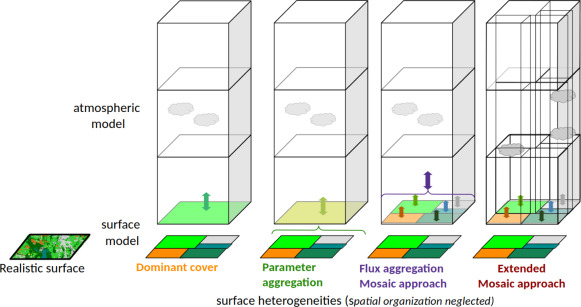
\includegraphics[width=0.8\textwidth]{images/mosaic_approach.jpg}
    \caption{ Conceptual view of the different paradigms to represent the land-atmosphere coupling over heterogeneous surface in models, from the simplest on the left to the more complex to the right. Note that the spatial organization of the heterogeneity and horizontal scale of the different patches are not taken into account. Taken from \citet{lohou_model_2025}}
    \label{fig:mosaic_approach}
\end{figure}

%the end